% CRME Evidence-Backed Results Package
% Automatically generated by PaperPackageBuilder

\section{Results}

The CRME evaluation pipeline was conducted across two datasets using five evaluation metrics.

The comparative evaluation identified SRCB\_v1 as the best-performing dataset across all reported metrics.

\begin{table}[htbp]
\centering
\caption{Baseline Performance of CRME}
\label{tab:crme-baseline-performance}
\begin{tabular}{lc}
\toprule
Metric & Score \\
\midrule
MCS & 47.50 \\
SRS & 100 \\
KGQ & 40.00 \\
RRS & 43.33 \\
CES & 57.71 \\
\bottomrule
\end{tabular}
\end{table}

\section{Ablation Study}

The ablation analysis evaluated the contribution of four architectural components under five configurations.

The decisions component exhibited the largest aggregate degradation, followed by relations, sessions, and artifacts.

\begin{table}[htbp]
\centering
\caption{Component Contribution Based on Ablation Analysis}
\label{tab:crme-ablation-ranking}
\begin{tabular}{lcc}
\toprule
Rank & Component & Aggregate Degradation \\
\midrule
1 & Decisions & 52.08 \\
2 & Relations & 50.00 \\
3 & Sessions & 20.83 \\
4 & Artifacts & 9.38 \\
\bottomrule
\end{tabular}
\end{table}

\begin{figure}[htbp]
\centering
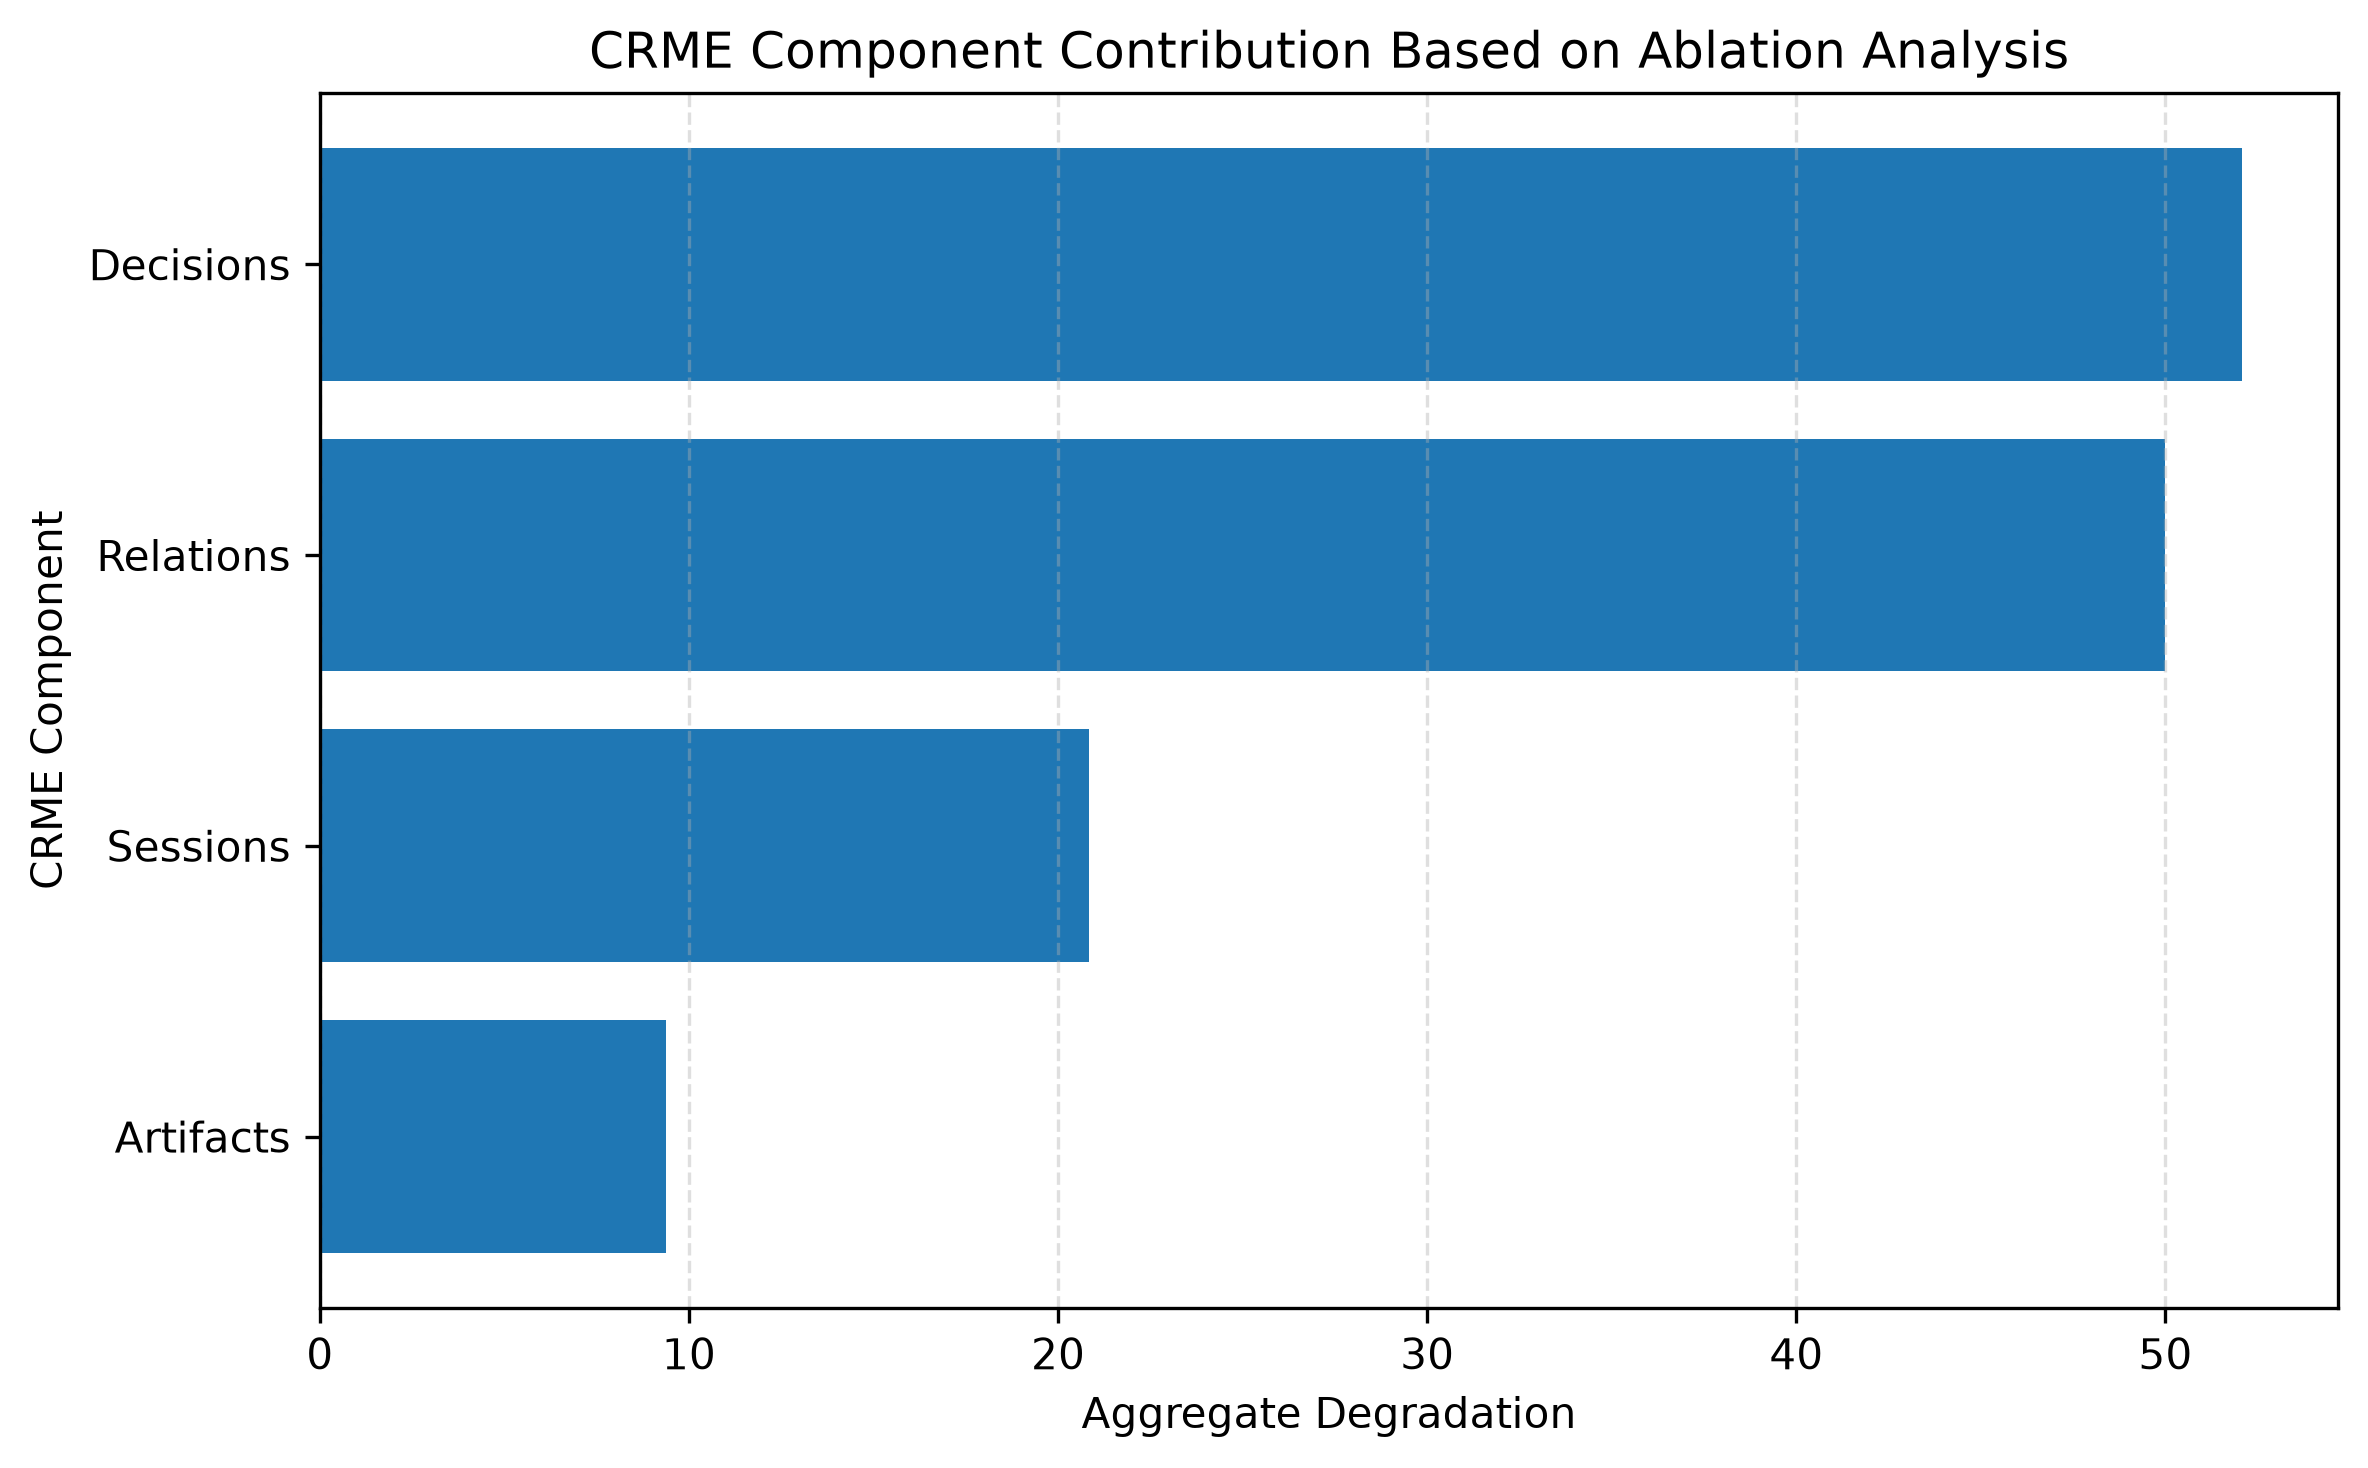
\includegraphics[width=0.8\linewidth]{figures/component_contribution_ranking.png}
\caption{Component contribution ranking based on aggregate ablation degradation.}
\label{fig:crme-component-contribution}
\end{figure}

\section{Statistical Analysis}

The current evaluation package reports descriptive baseline metrics and component-level degradation values.

No inferential statistical test, confidence interval, or hypothesis test is currently included in the evidence package.

Accordingly, the present results should be interpreted as descriptive and comparative rather than as statistically significant evidence of superiority over a baseline.

\section{Discussion}

The largest observed aggregate degradation was associated with the decisions component, whereas the artifacts component exhibited the lowest observed aggregate degradation.

These results indicate heterogeneous component contribution within the evaluated CRME architecture.

However, the observed ranking should be interpreted as an empirical comparative result rather than a definitive causal decomposition.

\section{Threats to Validity}

The current evidence package does not include inferential statistical testing or confidence interval estimation.

The ablation results provide comparative evidence of component contribution but do not establish definitive causal importance.

Generalization to other datasets and research workflows requires further validation.

\section{Reproducibility}

All reported results are derived from stored CRME evaluation artifacts.

The evaluation pipeline preserves the relationship between raw evidence, aggregated summaries, paper tables, figures, and claim-level evidence.

The Q1 consistency audit completed with overall status \texttt{PASS}.

Raw evaluation outputs are preserved and are not modified by the paper generation layer.
